\chapter{Literatura}


\begin{figure}[h!]
    \centering
    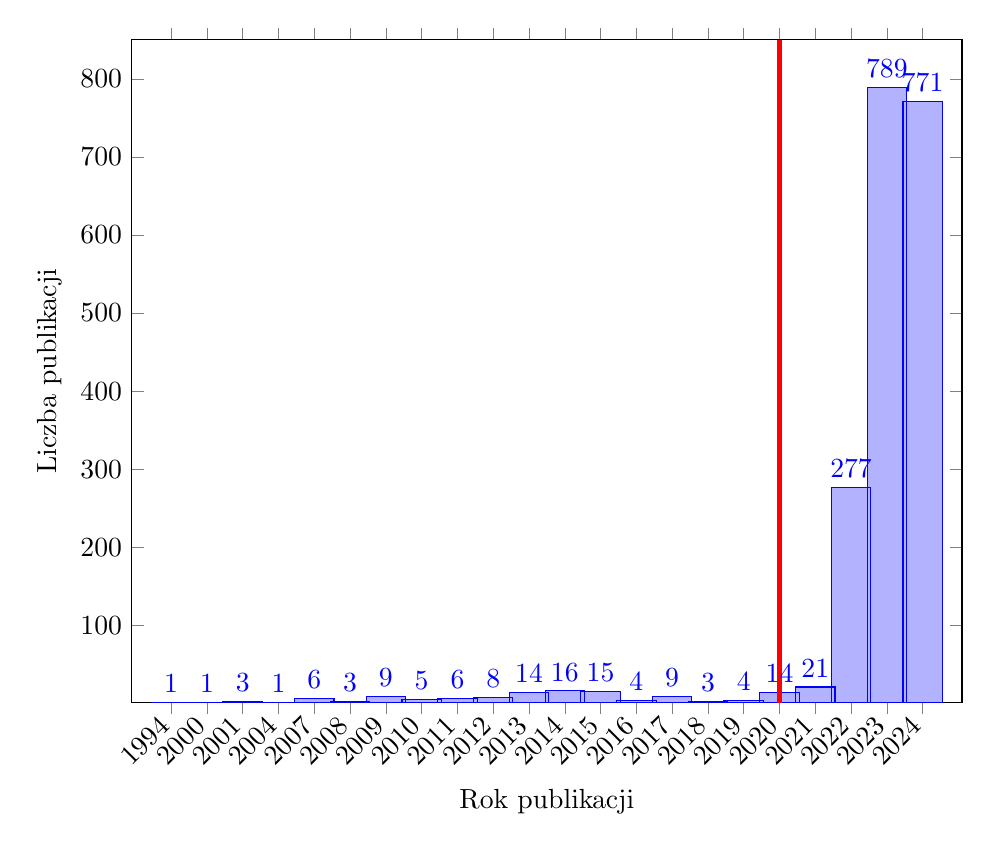
\begin{tikzpicture}
        \begin{axis}[
            width=\textwidth, height=10cm,
            xlabel={Rok publikacji},
            ylabel={Liczba publikacji},
            symbolic x coords={1994, 2000, 2001, 2004, 2007, 2008, 2009, 2010, 2011, 2012, 2013, 2014, 2015, 2016, 2017, 2018, 2019, 2020, 2021, 2022, 2023, 2024},
            xtick=data,
            ymin=1, ymax=850,
            ybar,
            bar width=0.5cm,
            nodes near coords,
            xticklabel style={rotate=45, anchor=east},
            enlarge x limits={abs=0.5cm}
        ]
        \addplot coordinates {(1994,1) (2000,1) (2001,3) (2004,1) (2007,6) (2008,3) (2009,9) (2010,5) (2011,6) (2012,8) (2013,14) (2014,16) (2015,15) (2016,4) (2017,9) (2018,3) (2019,4) (2020,14) (2021,21) (2022,277) (2023,789) (2024,771)};

        % Adding the horizontal line at year 2020
        \draw [red, ultra thick] (axis cs:2020,0) -- (axis cs:2020,850);
        
        \end{axis}
    \end{tikzpicture}
    \caption{Rozkład publikowania artykułów o tematyce Metaverse na przestrzeni lat }
    \label{fig:enter-label}
\end{figure}